\section{Gewichtsmatrizen} \label{gewichtsmatrizenSection}
In diesem Abschnitt werden verschiedene Gewichtsmatrizen vorgestellt und wie wir sie erzeugt haben. Wir haben uns erst einmal auf die Erzeugung mit der Gauß-Funktion konzentriert. Es sind auch andere Funktionen möglich, wie zum Beispiel die Rayleigh-Funktion. Aus zeitlichen Gründen mussten wie darauf leider verzichten.

Zuerst soll gezeigt werden, wie die Gewichtsmatrizen grob erstellt wurden. Dafür werden im Abschnitt \ref{eGew} 3 Beispiele mit jeweils einem Slope von 75 gezeigt. Es soll außerdem verdeutlicht werden, dass es sich immer nur um einen Gauß in x- und y-Richtung handelt. Des Weiteren ist das Endergebnis immer zwischen -1 und 1. So können wir später den Ergebnisbereich besser skalieren.

In den anderen Unter-Abschnitten sind für jede Art der Gewichtsmatrizen verschiedene Slopes eingestellt.

\newpage
\subsection{Erzeugung der Gewichtsmatrizen} \label{eGew}
\begin{figure}[hbt]
	\centering
	\includegraphics[width=1\linewidth]{./Bilder/Auswertung/GewichtmatrixEinzelschritte/Endergebnis_Gewichtsmatrix_Slope_75_Type_Add}
	\caption{Additive Überlagerung mit Slope von 75}
	\label{Add75}
\end{figure}

\begin{lstlisting}[label=code:Add75, caption=Auszug Matlab-Skript 'GetGaussWeights()']
elseif strcmp(type, 'Add')
	for i = 1:vN
		tempWeightMatrix(1:end, i) = (vWeightMatrix(1:end, i) + (hGauss./max(hGauss))')./2;
		tempWeightMatrix(1:end, i) = tempWeightMatrix(1:end, i) .* 2 - 1;
	end
\end{lstlisting}

In Abbildung \ref{Add75} wurde der 3D-Gauß in x- und y-Richtung additiv Überlagert, mit 2 multipliziert und am Ende um 1 heruntergesetzt. Siehe auch das Listing \ref{code:Add75}.

\newpage
\begin{figure}[hbt]
	\centering
	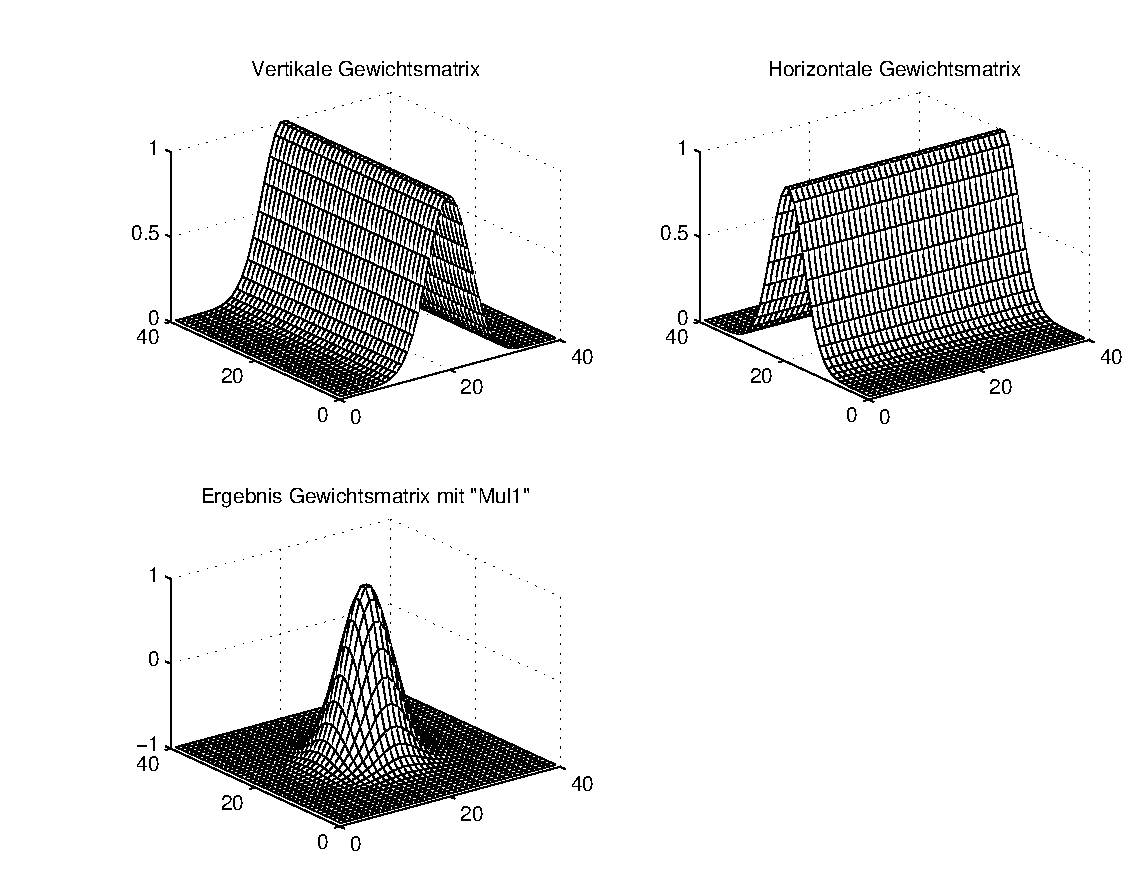
\includegraphics[width=1\linewidth]{./Bilder/Auswertung/GewichtmatrixEinzelschritte/Endergebnis_Gewichtsmatrix_Slope_75_Type_Mul1}
	\caption{Multiplikative Überlagerung Typ 1 mit Slope von 75}
	\label{Mul175}
\end{figure}

\begin{lstlisting}[label=code:Mul175, caption=Auszug Matlab-Skript 'GetGaussWeights()']
if strcmp(type, 'Mul1')
	for i = 1:vN
		tempWeightMatrix(1:end, i) = vWeightMatrix(1:end, i) .* (hGauss./max(hGauss))';
		tempWeightMatrix(1:end, i) = tempWeightMatrix(1:end, i) .* 2 - 1;
	end
\end{lstlisting}

In Abbildung \ref{Mul175} wurde der 3D-Gauß in x- und y-Richtung multiplikativ Überlagert, mit 2 multipliziert und am Ende um 1 heruntergesetzt. Siehe auch das Listing \ref{code:Mul175}.

\newpage
\begin{figure}[hbt]
	\centering
	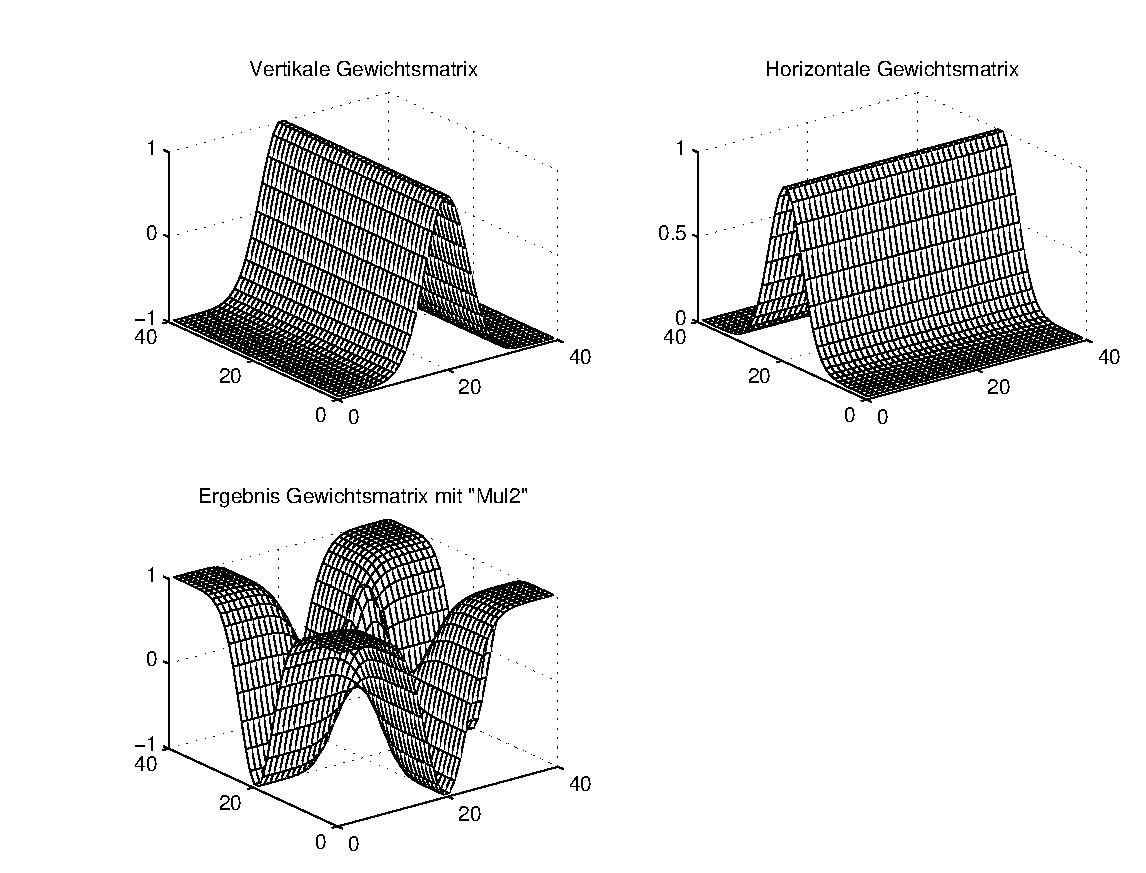
\includegraphics[width=1\linewidth]{./Bilder/Auswertung/GewichtmatrixEinzelschritte/Endergebnis_Gewichtsmatrix_Slope_75_Type_Mul2}
	\caption{Multiplikative Überlagerung Typ 2 mit Slope von 75}
	\label{Mul275}
\end{figure}

\begin{lstlisting}[label=code:Mul275, caption=Auszug Matlab-Skript 'GetGaussWeights()']
elseif strcmp(type, 'Mul2')
	for i = 1:vN
		% skalieren auf -1 bis 1
		vWeightMatrix(1:end, i) = vWeightMatrix(1:end, i) .* 2 - 1;
		% v-Gauss und h-Gauss multiplizieren
		tempWeightMatrix(1:end, i) = vWeightMatrix(1:end, i) .* ((hGauss./max(hGauss)) * 2 - 1)';
	end
\end{lstlisting}

In Abbildung \ref{Mul275} wurde der 3D-Gauß in der einen y-Richtung erst einmal zwischen -1 und 1 skaliert. Anschließend wird der 3D-Gauß in x-Richtung ebenfalls zwischen -1 und 1 skaliert. Am Ende werden beide multiplikativ überlagert. Siehe auch das Listing \ref{code:Mul275}.

\newpage
\subsection{Additive Überlagerung}
\begin{figure}[hbt]
	\begin{minipage}{0.5 \textwidth}
		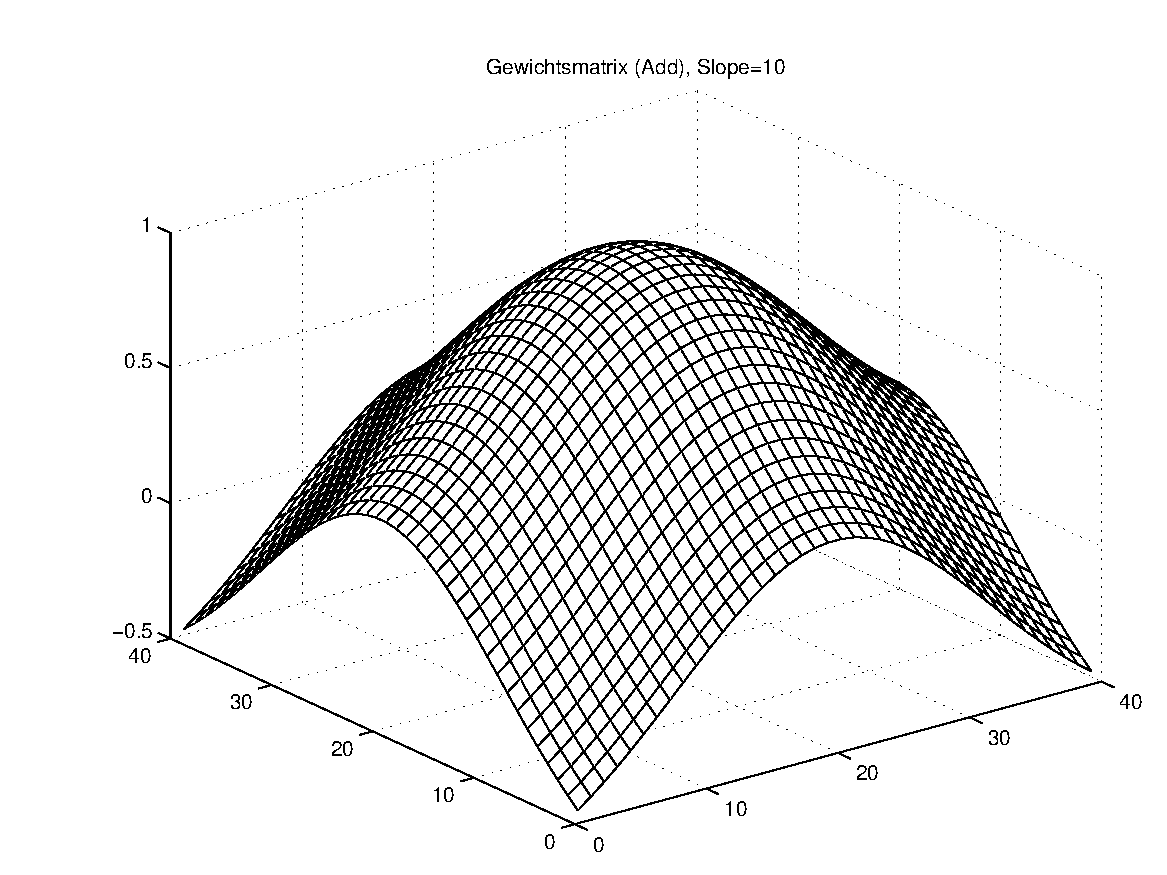
\includegraphics[width=\textwidth]{./Bilder/Auswertung/Gewichtsmatrix/Gewichtsmatrix_Add_Slope_10}
		\caption{Additive Überlagerung mit Slope von 10}
		\label{Add10}
	\end{minipage}
	\hfill
	\begin{minipage}{0.5 \textwidth}
		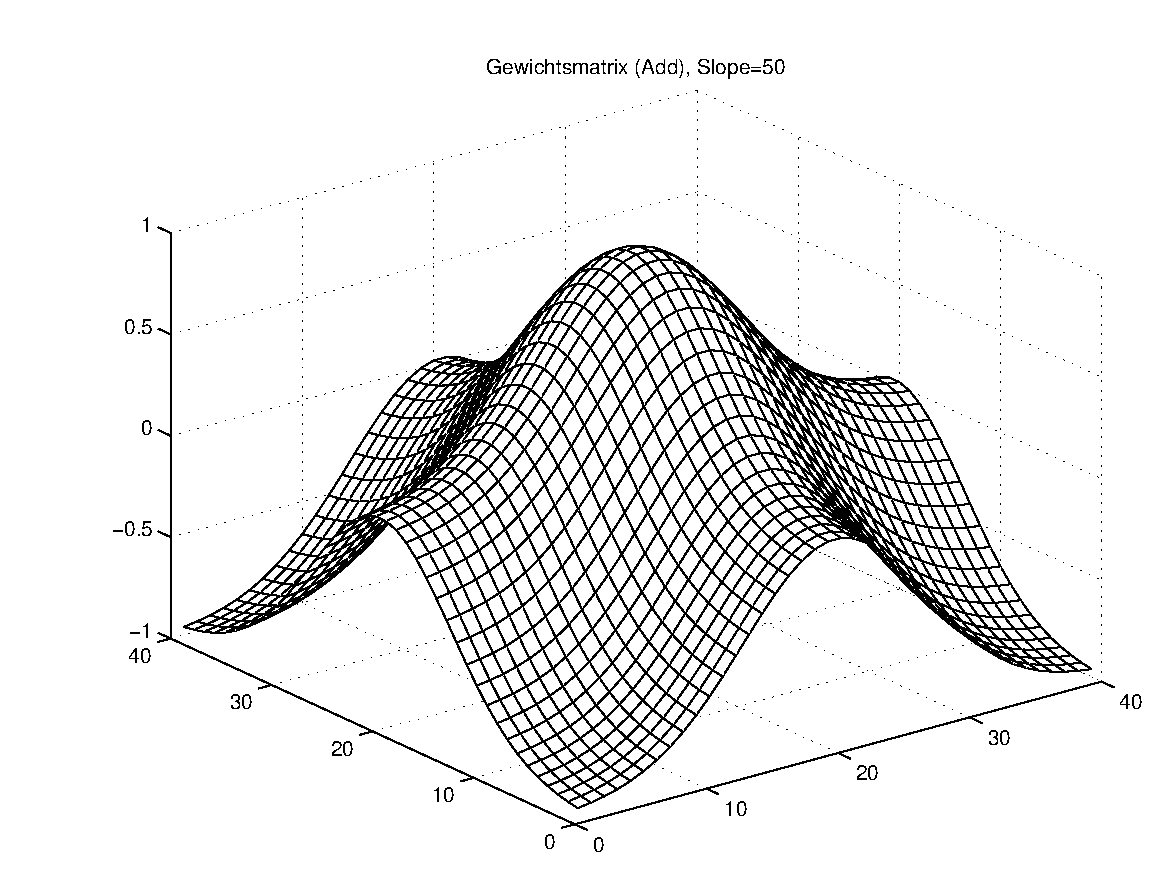
\includegraphics[width=\textwidth]{./Bilder/Auswertung/Gewichtsmatrix/Gewichtsmatrix_Add_Slope_50}
		\caption{Additive Überlagerung mit Slope von 50}
		\label{Add50}
	\end{minipage}
\end{figure}

\begin{figure}[hbt]
	\centering
	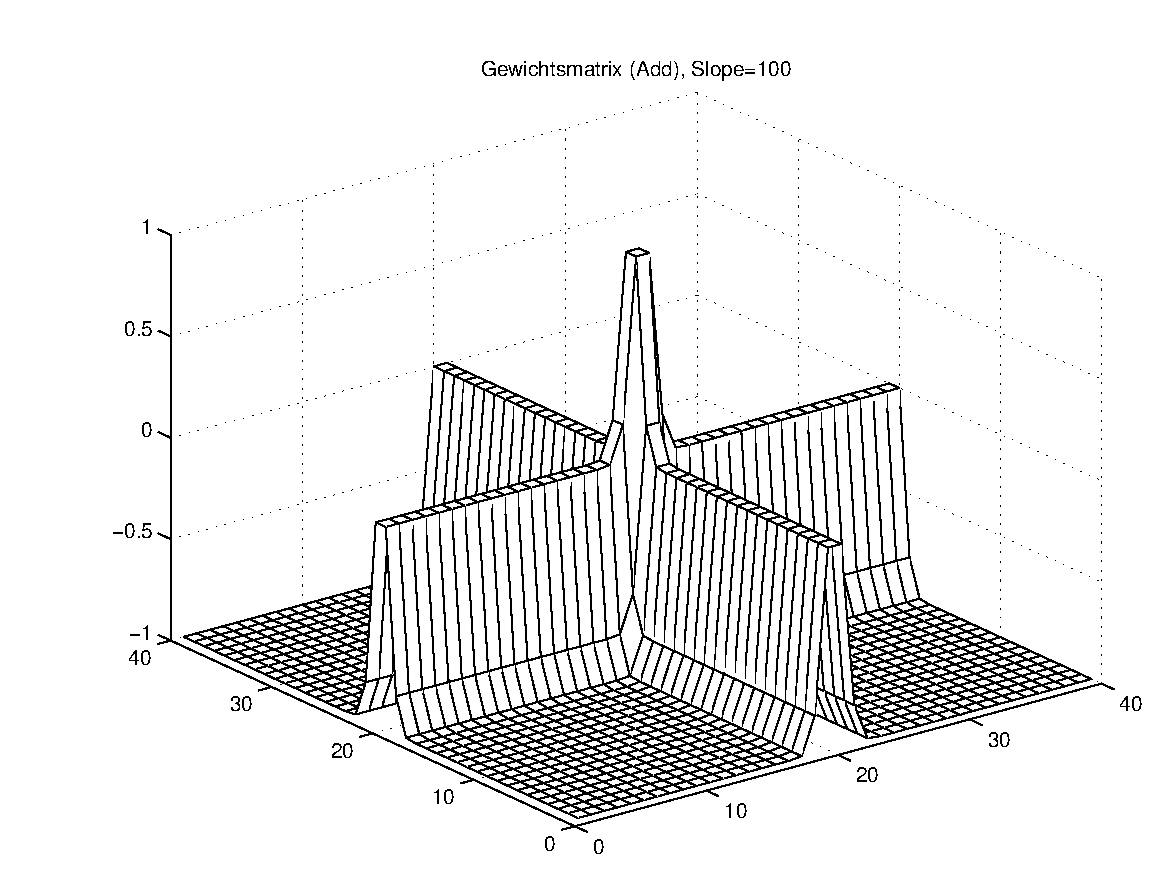
\includegraphics[width=0.6\linewidth]{./Bilder/Auswertung/Gewichtsmatrix/Gewichtsmatrix_Add_Slope_100}
	\caption{Additive Überlagerung mit Slope von 100}
	\label{Add100}
\end{figure}

\newpage
\subsection{Multiplikative Überlagerung Typ 1}
\begin{figure}[hbt]
	\begin{minipage}{0.5 \textwidth}
		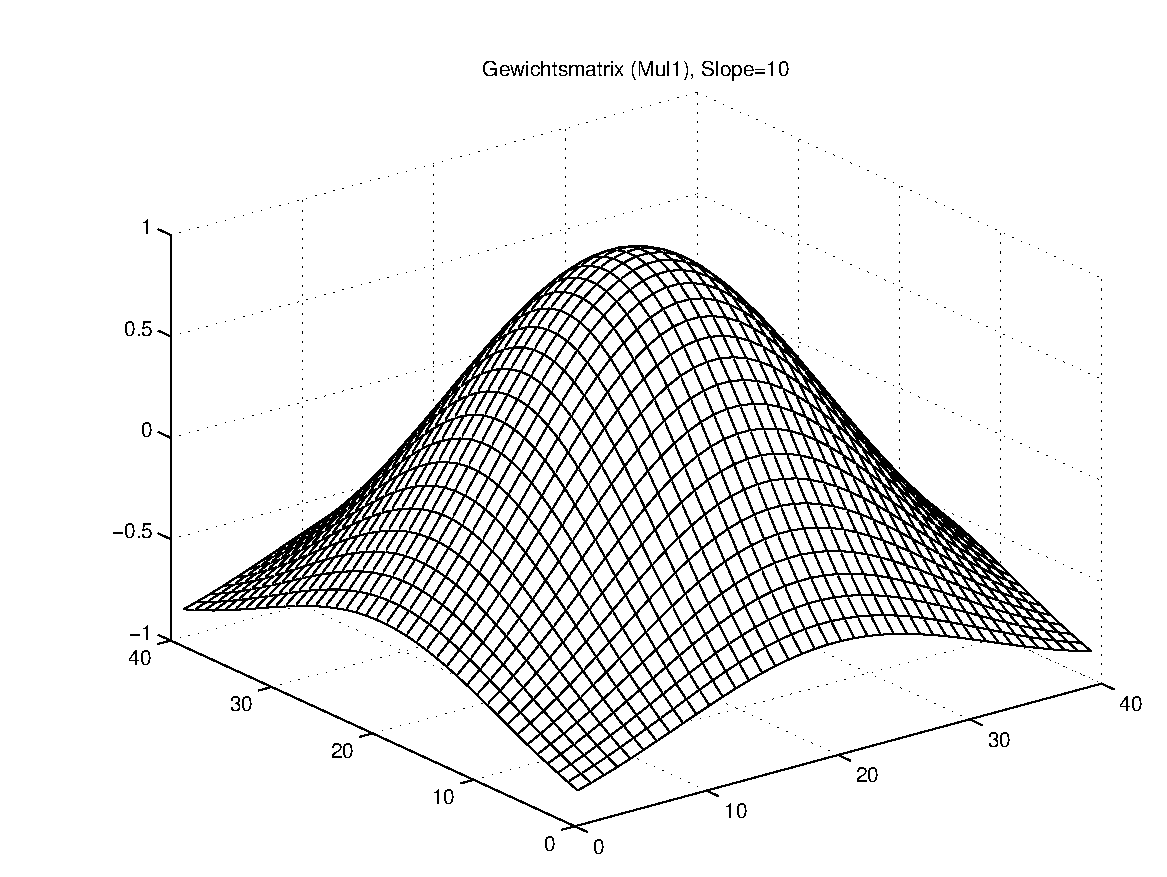
\includegraphics[width=\textwidth]{./Bilder/Auswertung/Gewichtsmatrix/Gewichtsmatrix_Mul1_Slope_10}
		\caption{Multiplikative Überlagerung Typ 1 mit Slope von 10}
		\label{Mul110}
	\end{minipage}
	\hfill
	\begin{minipage}{0.5 \textwidth}
		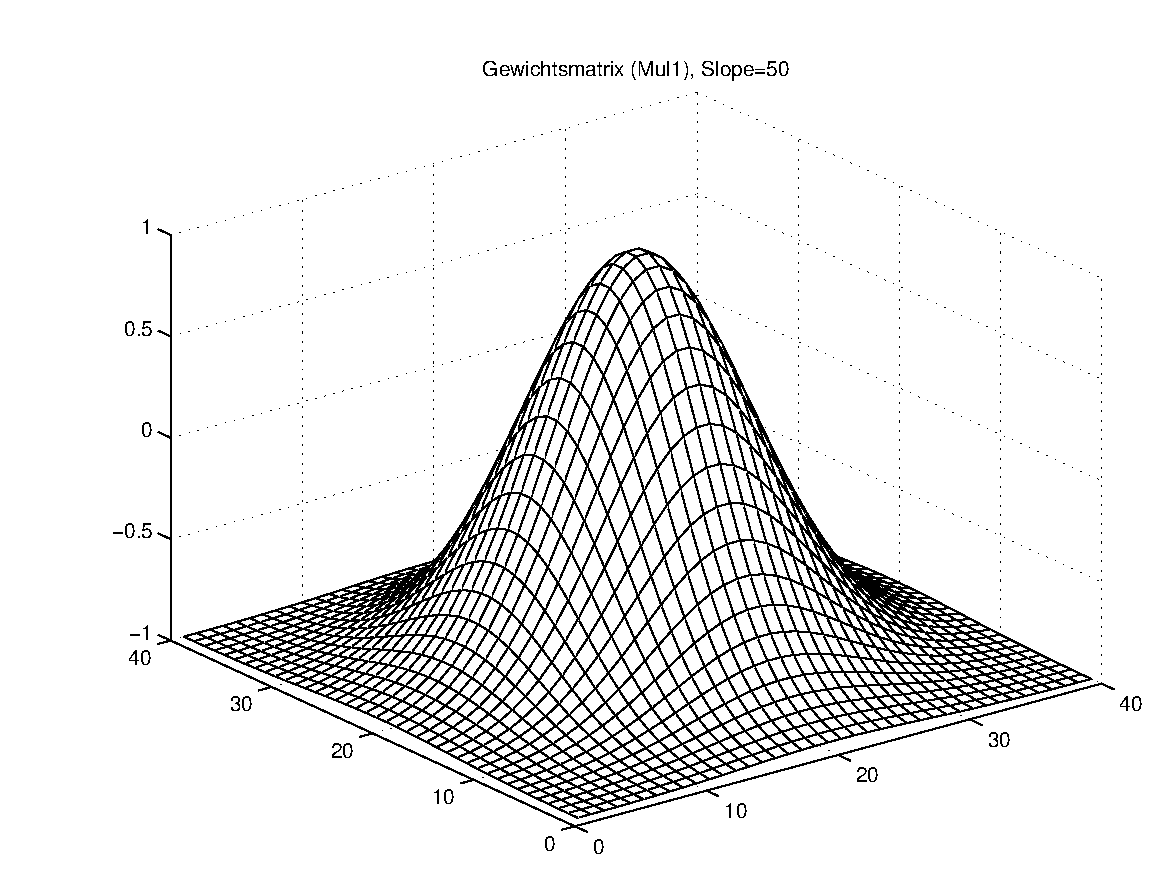
\includegraphics[width=\textwidth]{./Bilder/Auswertung/Gewichtsmatrix/Gewichtsmatrix_Mul1_Slope_50}
		\caption{Multiplikative Überlagerung Typ 1 mit Slope von 50}
		\label{Mul150}
	\end{minipage}
\end{figure}

\begin{figure}[hbt]
	\centering
	\includegraphics[width=0.6\linewidth]{./Bilder/Auswertung/Gewichtsmatrix/Gewichtsmatrix_Mul1_Slope_100}
	\caption{Multiplikative Überlagerung Typ 1 mit Slope von 100}
	\label{Mul1100}
\end{figure}

\newpage
\subsection{Multiplikative Überlagerung Typ 2}
\begin{figure}[hbt]
	\begin{minipage}{0.5 \textwidth}
		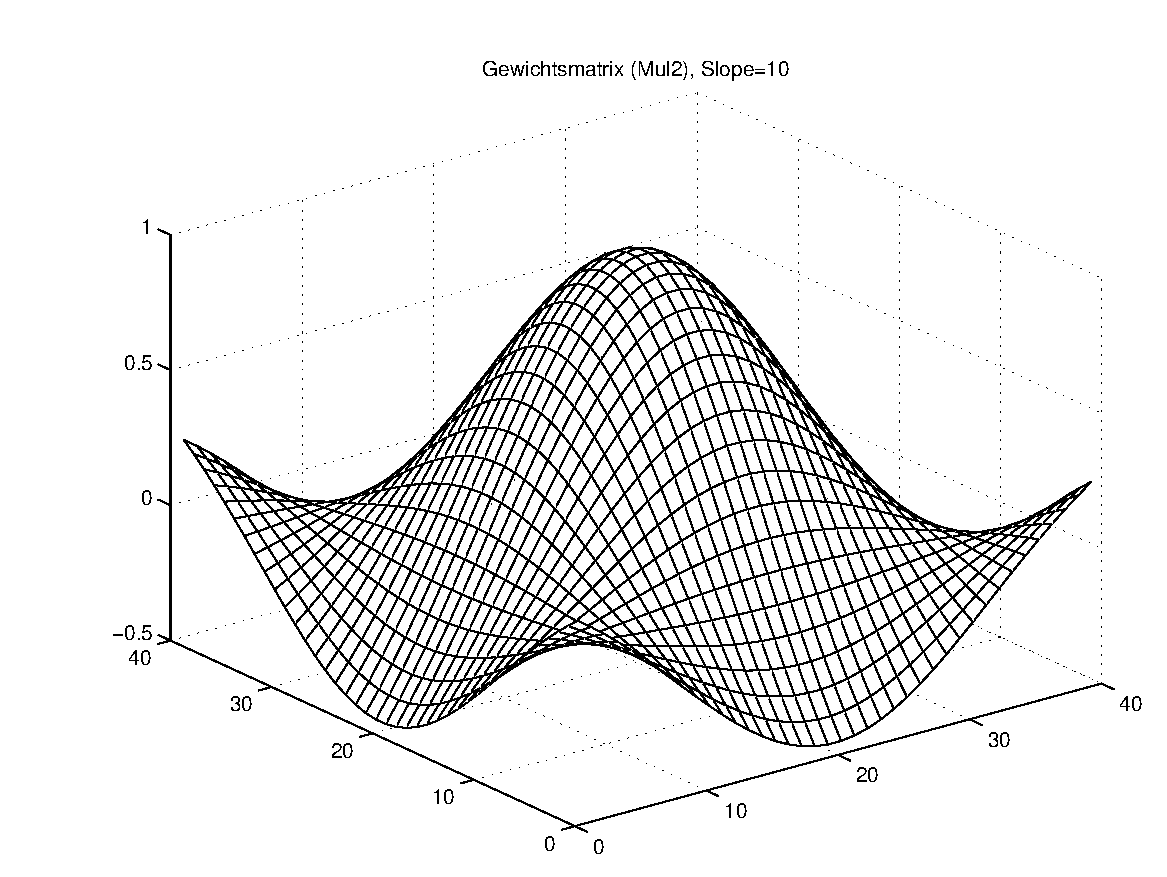
\includegraphics[width=\textwidth]{./Bilder/Auswertung/Gewichtsmatrix/Gewichtsmatrix_Mul2_Slope_10}
		\caption{Multiplikative Überlagerung Typ 2 mit Slope von 10}
		\label{Mul210}
	\end{minipage}
	\hfill
	\begin{minipage}{0.5 \textwidth}
		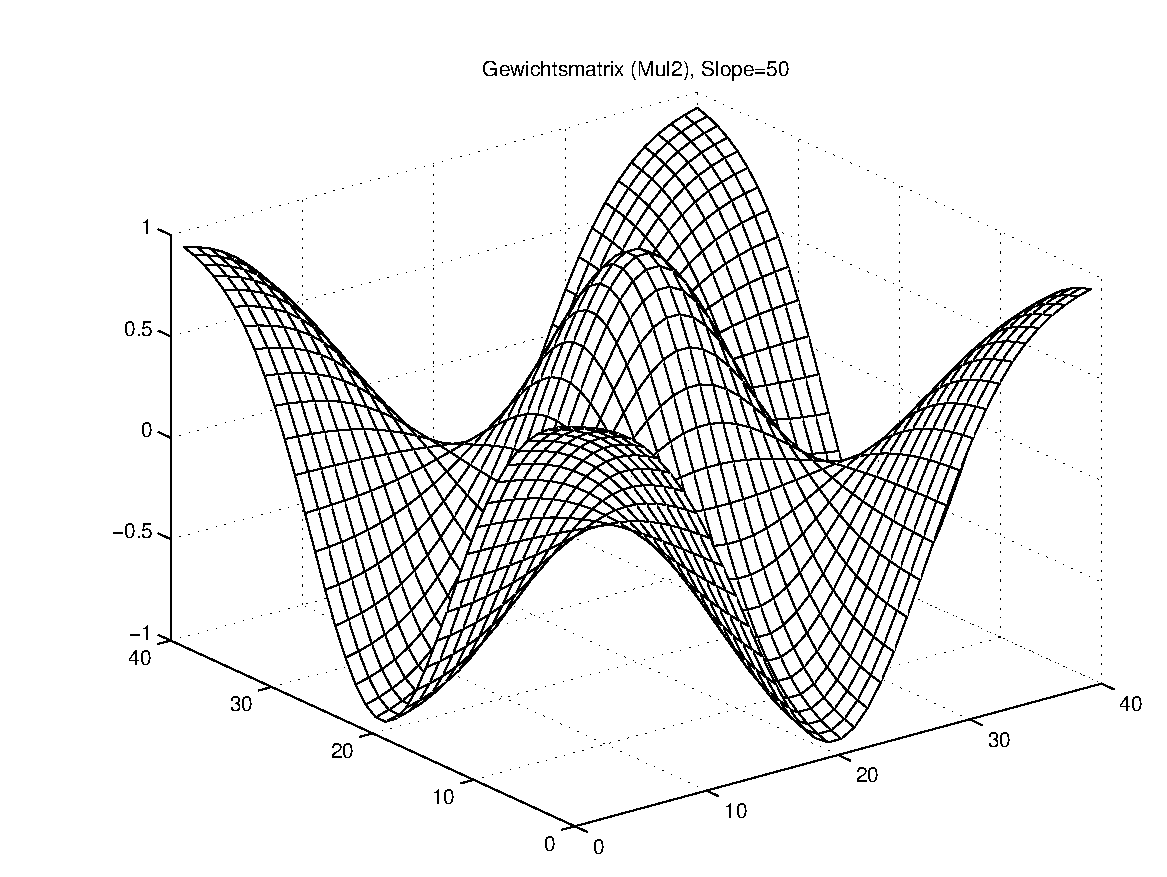
\includegraphics[width=\textwidth]{./Bilder/Auswertung/Gewichtsmatrix/Gewichtsmatrix_Mul2_Slope_50}
		\caption{Multiplikative Überlagerung Typ 2 mit Slope von 50}
		\label{Mul250}
	\end{minipage}
\end{figure}

\begin{figure}[hbt]
	\centering
	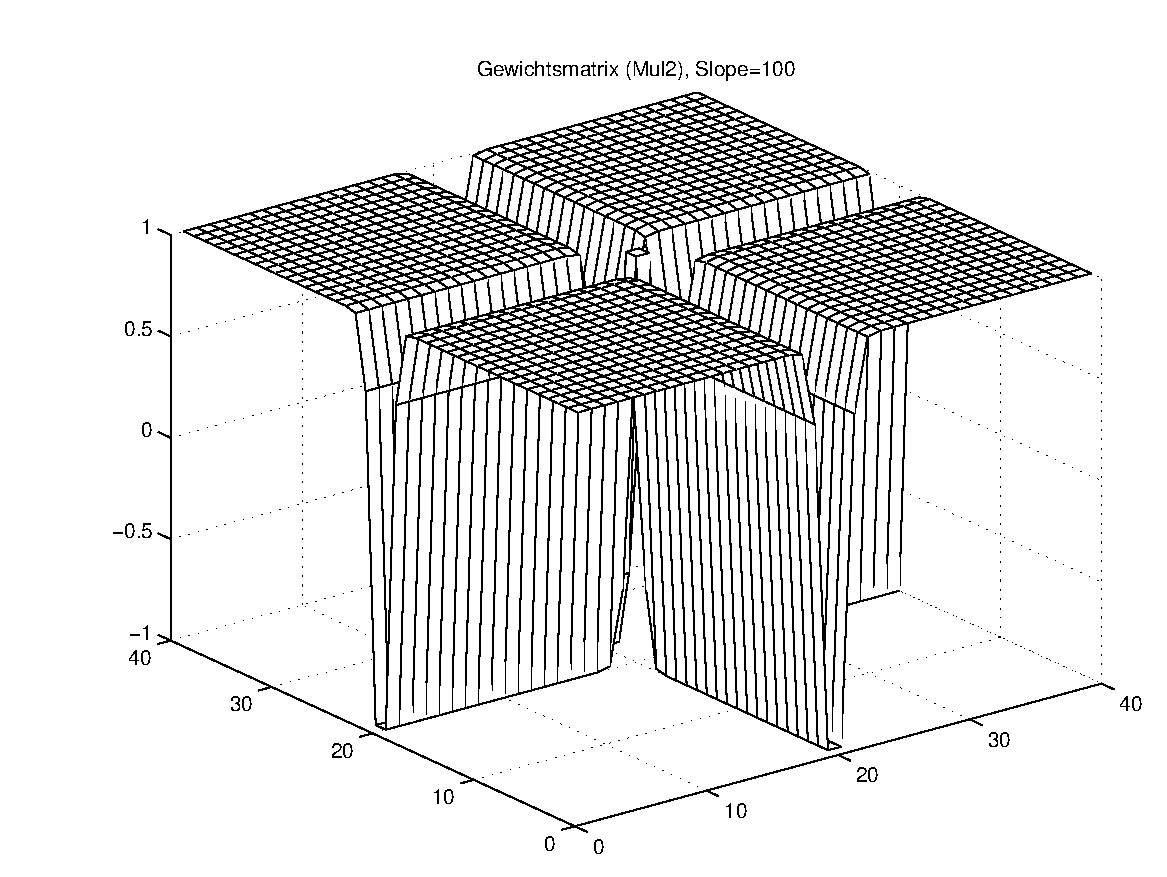
\includegraphics[width=0.6\linewidth]{./Bilder/Auswertung/Gewichtsmatrix/Gewichtsmatrix_Mul2_Slope_100}
	\caption{Multiplikative Überlagerung Typ 2 mit Slope von 100}
	\label{Mul2100}
\end{figure}


\newpage
\subsection{Additive und Multiplikative Überlagerung}
\begin{figure}[hbt]
	\begin{minipage}{0.5 \textwidth}
		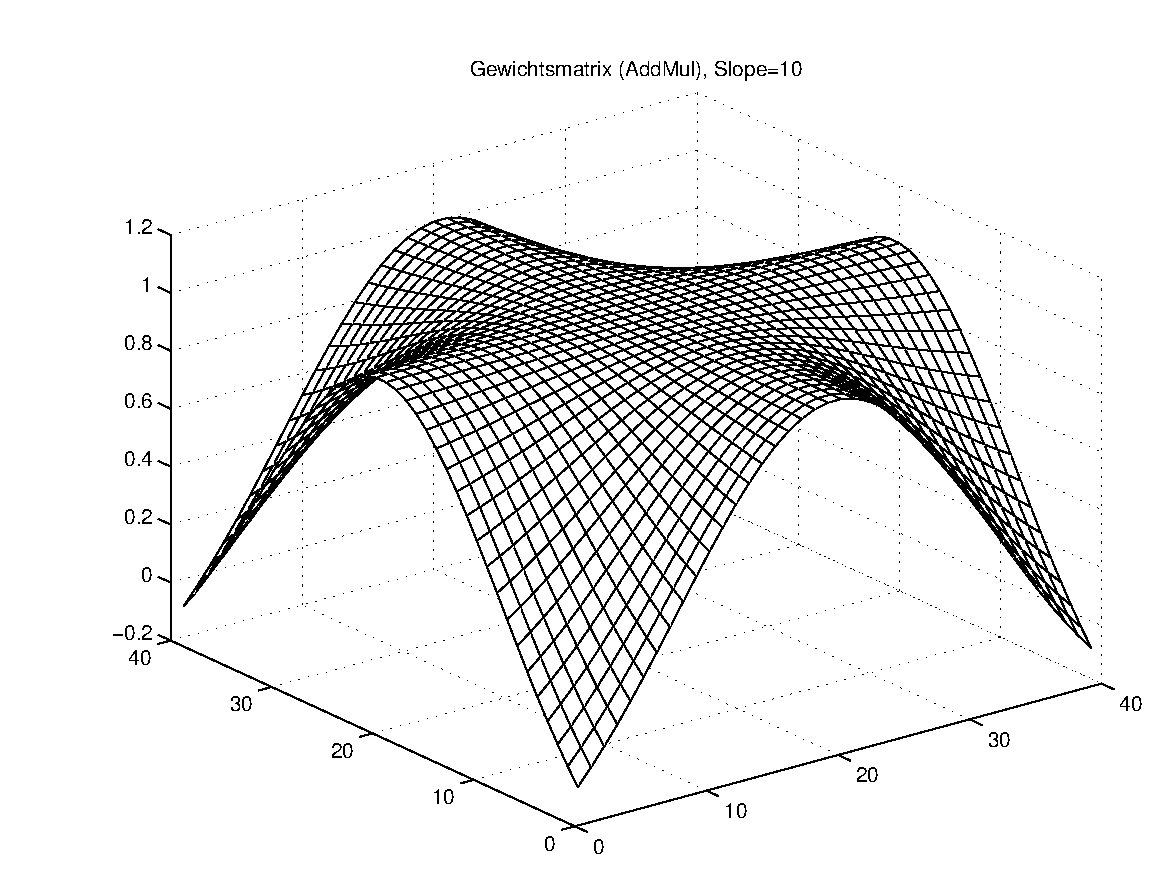
\includegraphics[width=\textwidth]{./Bilder/Auswertung/Gewichtsmatrix/Gewichtsmatrix_AddMul_Slope_10}
		\caption{Additive und Multiplikative Überlagerung mit Slope von 10}
		\label{AddMul210}
	\end{minipage}
	\hfill
	\begin{minipage}{0.5 \textwidth}
		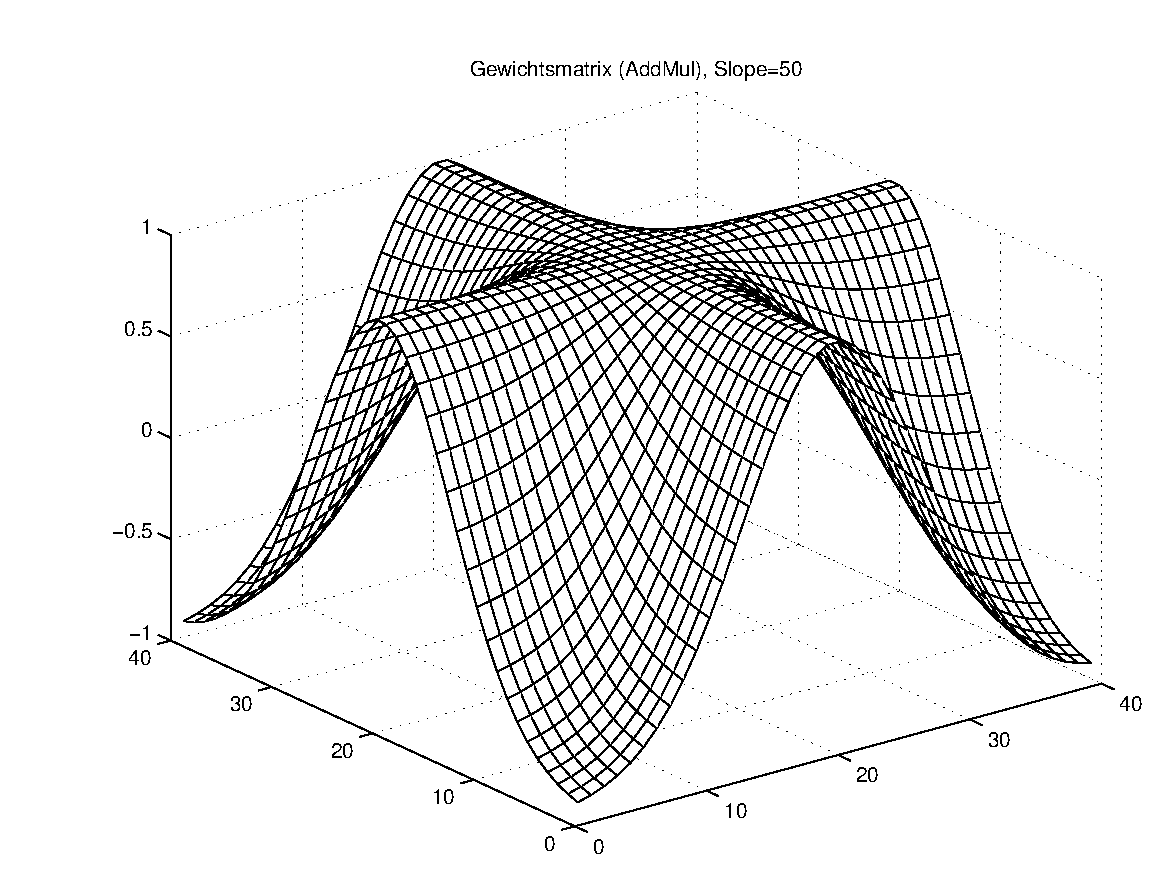
\includegraphics[width=\textwidth]{./Bilder/Auswertung/Gewichtsmatrix/Gewichtsmatrix_AddMul_Slope_50}
		\caption{Additive und Multiplikative Überlagerung mit Slope von 50}
		\label{AddMul50}
	\end{minipage}
\end{figure}

\begin{figure}[hbt]
	\centering
	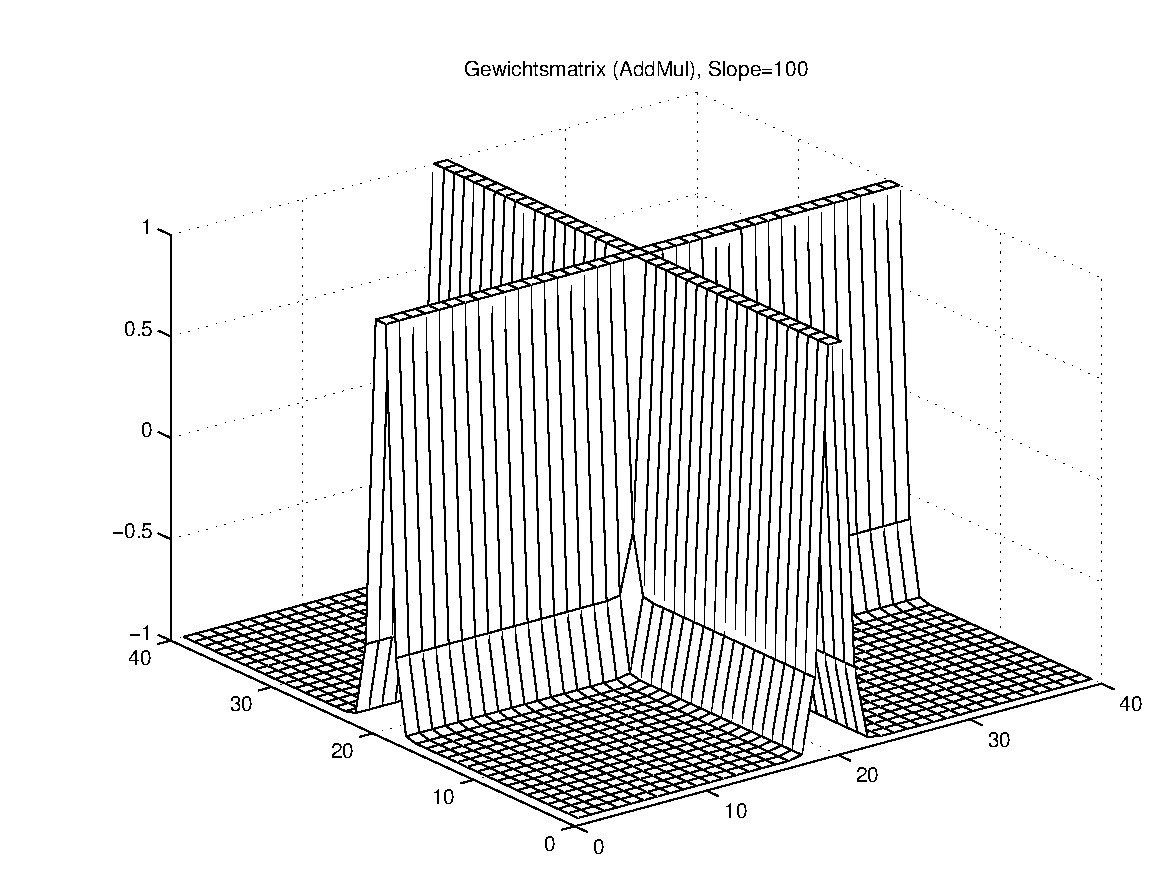
\includegraphics[width=0.6\linewidth]{./Bilder/Auswertung/Gewichtsmatrix/Gewichtsmatrix_AddMul_Slope_100}
	\caption{Additive und Multiplikative Überlagerung mit Slope von 100}
	\label{AddMul100}
\end{figure}

\newpage
\subsection{Spezielle Überlagerung}
\begin{figure}[hbt]
	\begin{minipage}{0.5 \textwidth}
		\includegraphics[width=\textwidth]{./Bilder/Auswertung/Gewichtsmatrix/Gewichtsmatrix_Special_Slope_10}
		\caption{Spezielle Überlagerung mit Slope von 10}
		\label{Spez210}
	\end{minipage}
	\hfill
	\begin{minipage}{0.5 \textwidth}
		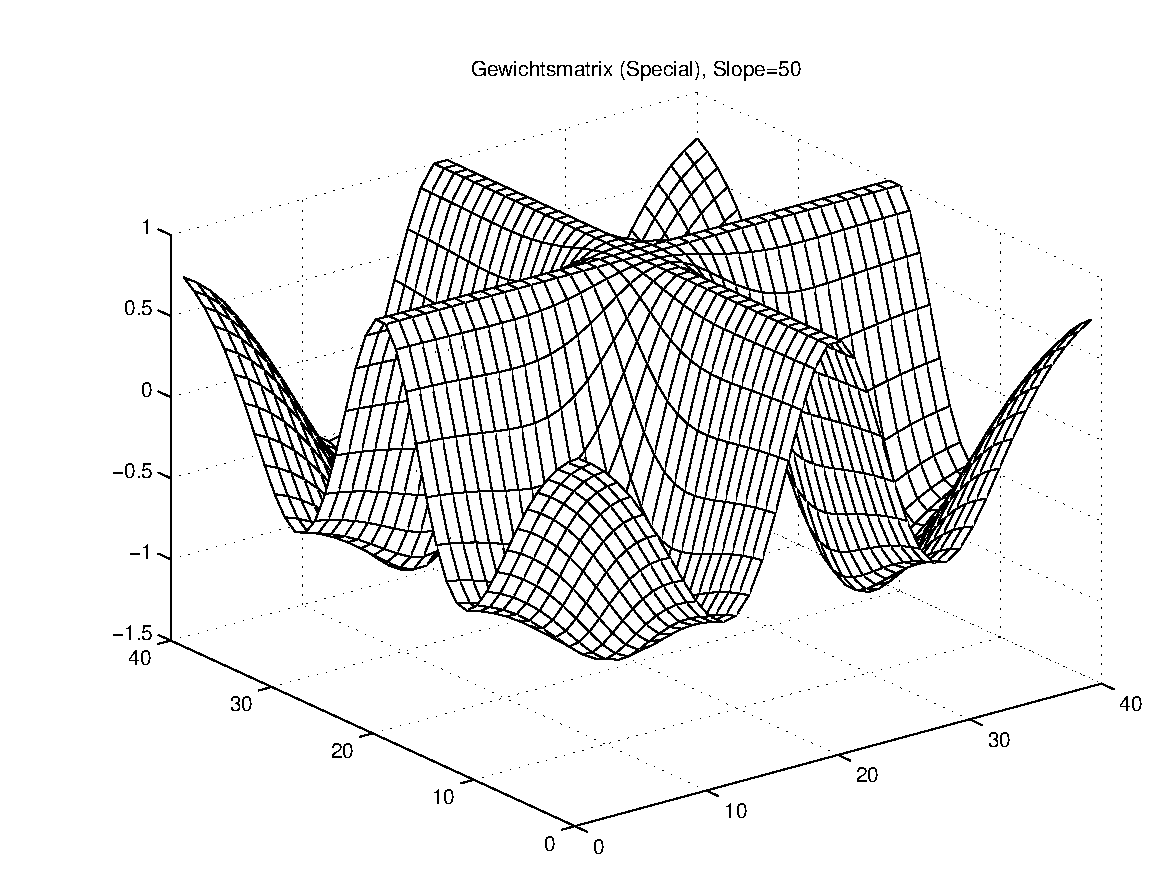
\includegraphics[width=\textwidth]{./Bilder/Auswertung/Gewichtsmatrix/Gewichtsmatrix_Special_Slope_50}
		\caption{Spezielle Überlagerung mit Slope von 50}
		\label{Spezl50}
	\end{minipage}
\end{figure}

\begin{figure}[hbt]
	\centering
	\includegraphics[width=0.6\linewidth]{./Bilder/Auswertung/Gewichtsmatrix/Gewichtsmatrix_Special_Slope_100}
	\caption{Spezielle Überlagerung mit Slope von 100}
	\label{Spez100}
\end{figure}

Bei der Speziellen Gewichtsmatrix hat der Slope keine Auswirkungen. Das war viel mehr ein Versuch, die Auswirkung von erhöhten Gewichten in den Randbereichen zu untersuchen. Aus diesen Grund wurde sie empirisch ermittelt aus den Typen: 'Mul1', 'Mul2' und 'AddMul'.